% Options for packages loaded elsewhere
\PassOptionsToPackage{unicode}{hyperref}
\PassOptionsToPackage{hyphens}{url}
%
\documentclass[
]{article}
\usepackage{amsmath,amssymb}
\usepackage{iftex}
\ifPDFTeX
  \usepackage[T1]{fontenc}
  \usepackage[utf8]{inputenc}
  \usepackage{textcomp} % provide euro and other symbols
\else % if luatex or xetex
  \usepackage{unicode-math} % this also loads fontspec
  \defaultfontfeatures{Scale=MatchLowercase}
  \defaultfontfeatures[\rmfamily]{Ligatures=TeX,Scale=1}
\fi
\usepackage{lmodern}
\ifPDFTeX\else
  % xetex/luatex font selection
\fi
% Use upquote if available, for straight quotes in verbatim environments
\IfFileExists{upquote.sty}{\usepackage{upquote}}{}
\IfFileExists{microtype.sty}{% use microtype if available
  \usepackage[]{microtype}
  \UseMicrotypeSet[protrusion]{basicmath} % disable protrusion for tt fonts
}{}
\makeatletter
\@ifundefined{KOMAClassName}{% if non-KOMA class
  \IfFileExists{parskip.sty}{%
    \usepackage{parskip}
  }{% else
    \setlength{\parindent}{0pt}
    \setlength{\parskip}{6pt plus 2pt minus 1pt}}
}{% if KOMA class
  \KOMAoptions{parskip=half}}
\makeatother
\usepackage{xcolor}
\usepackage[margin=1in]{geometry}
\usepackage{graphicx}
\makeatletter
\def\maxwidth{\ifdim\Gin@nat@width>\linewidth\linewidth\else\Gin@nat@width\fi}
\def\maxheight{\ifdim\Gin@nat@height>\textheight\textheight\else\Gin@nat@height\fi}
\makeatother
% Scale images if necessary, so that they will not overflow the page
% margins by default, and it is still possible to overwrite the defaults
% using explicit options in \includegraphics[width, height, ...]{}
\setkeys{Gin}{width=\maxwidth,height=\maxheight,keepaspectratio}
% Set default figure placement to htbp
\makeatletter
\def\fps@figure{htbp}
\makeatother
\setlength{\emergencystretch}{3em} % prevent overfull lines
\providecommand{\tightlist}{%
  \setlength{\itemsep}{0pt}\setlength{\parskip}{0pt}}
\setcounter{secnumdepth}{-\maxdimen} % remove section numbering
\ifLuaTeX
  \usepackage{selnolig}  % disable illegal ligatures
\fi
\usepackage{bookmark}
\IfFileExists{xurl.sty}{\usepackage{xurl}}{} % add URL line breaks if available
\urlstyle{same}
\hypersetup{
  pdftitle={Studentenfeedback-Bericht},
  hidelinks,
  pdfcreator={LaTeX via pandoc}}

\title{Studentenfeedback-Bericht}
\author{}
\date{\vspace{-2.5em}}

\begin{document}
\maketitle

In diesem Bericht wird das Feedback der Studierenden zu verschiedenen
Aspekten des Lehrangebots ausgewertet, um Verbesserungsansätze zu
identifizieren. Die allgemeine Zufriedenheit ist überwiegend hoch;
dennoch gibt es Bereiche, in denen sich die Studierenden
Weiterentwicklungen wünschen.

\subsection{Zufriedenheit mit Vorlesungen und
Übungen}\label{zufriedenheit-mit-vorlesungen-und-uxfcbungen}

Die Mehrheit der Studierenden bewertet die Vorlesungen positiv,
besonders hinsichtlich Struktur und Inhalt. Einige wünschen sich jedoch
mehr Interaktivität zur besseren Festigung der Inhalte. Auch die
Übungsgruppen erhalten gutes Feedback, allerdings äußerten manche den
Wunsch nach kleineren Gruppen und einer besseren Betreuung.

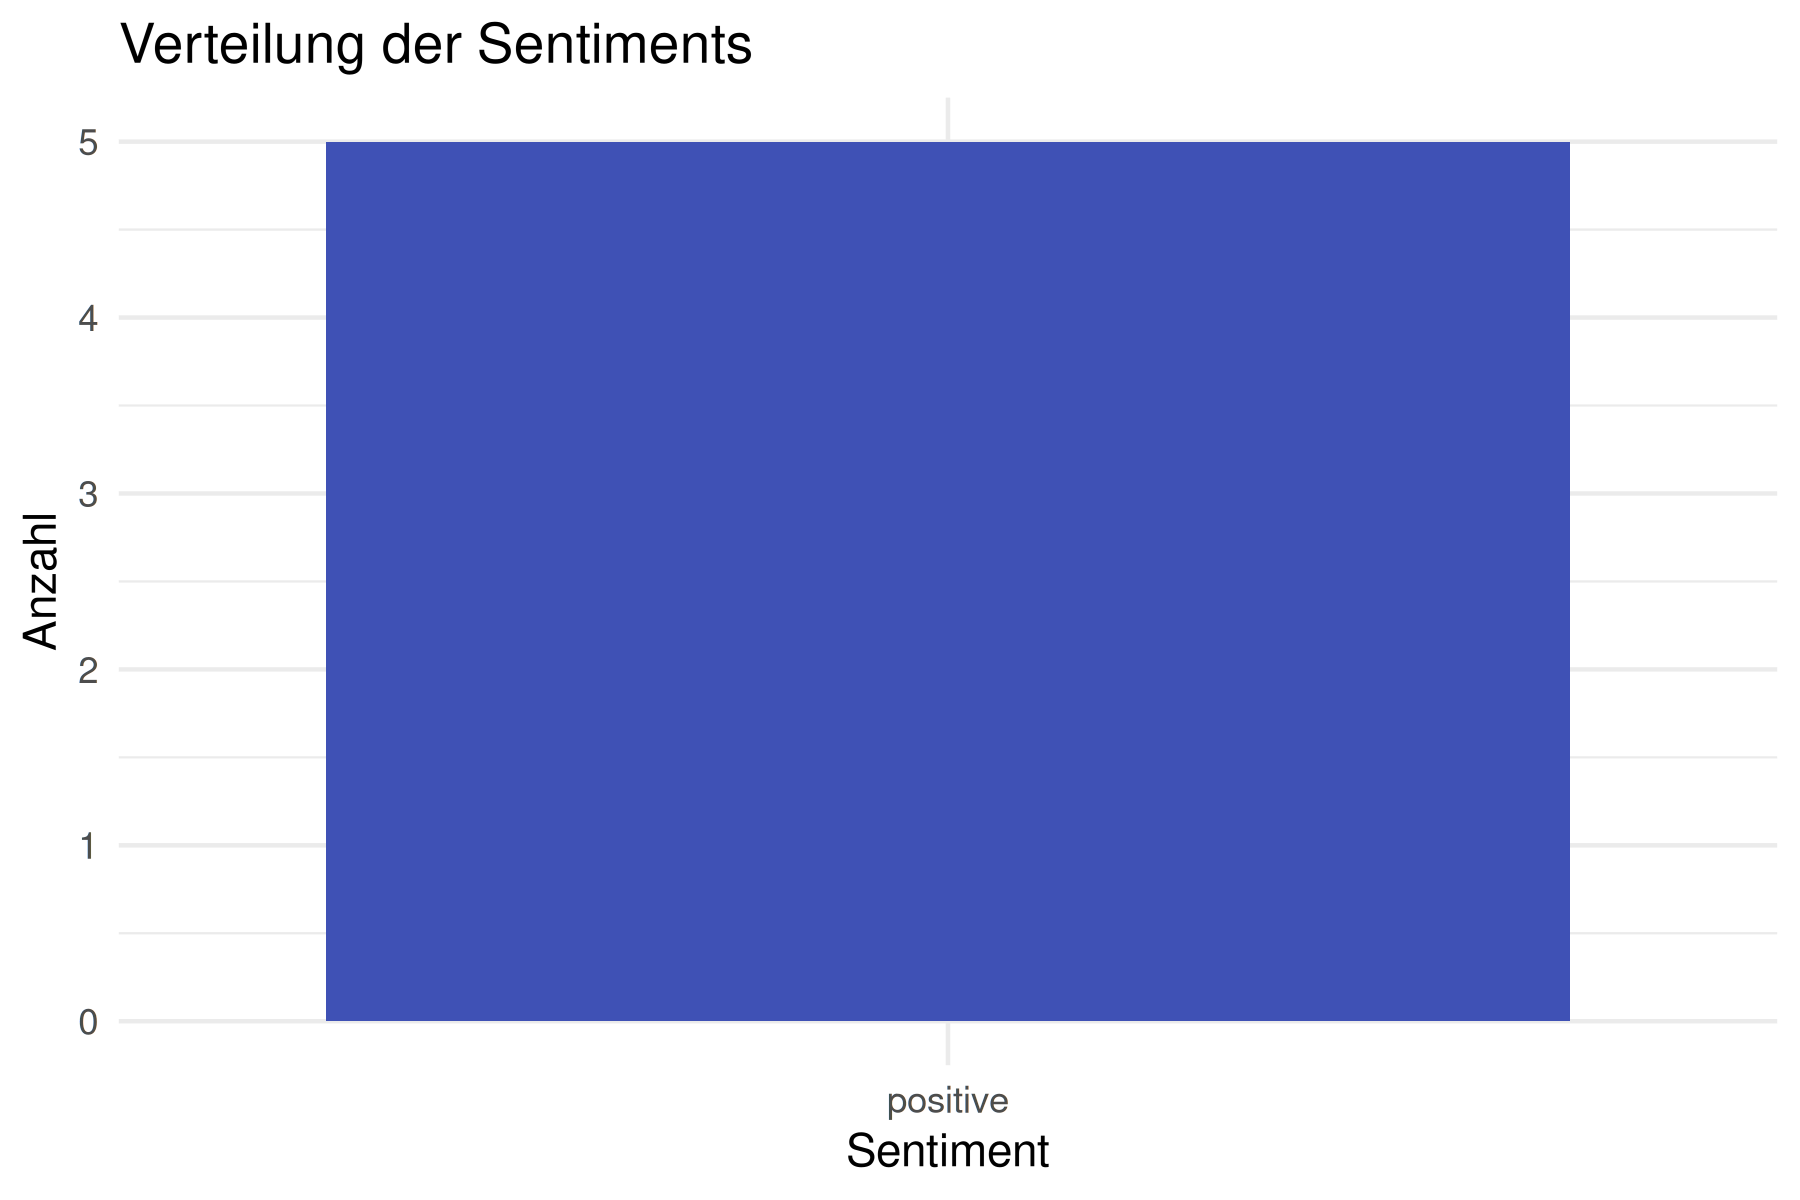
\includegraphics{Analyse_Diagramm1.png}

\subsection{Unterstützung durch
Lehrende}\label{unterstuxfctzung-durch-lehrende}

Die Unterstützung und Zugänglichkeit der Lehrenden werden generell als
sehr gut wahrgenommen. Studierende schätzen die schnelle Reaktion auf
Anfragen. Ein kleines Verbesserungspotenzial liegt in der Erweiterung
der digitalen Betreuungsmöglichkeiten.

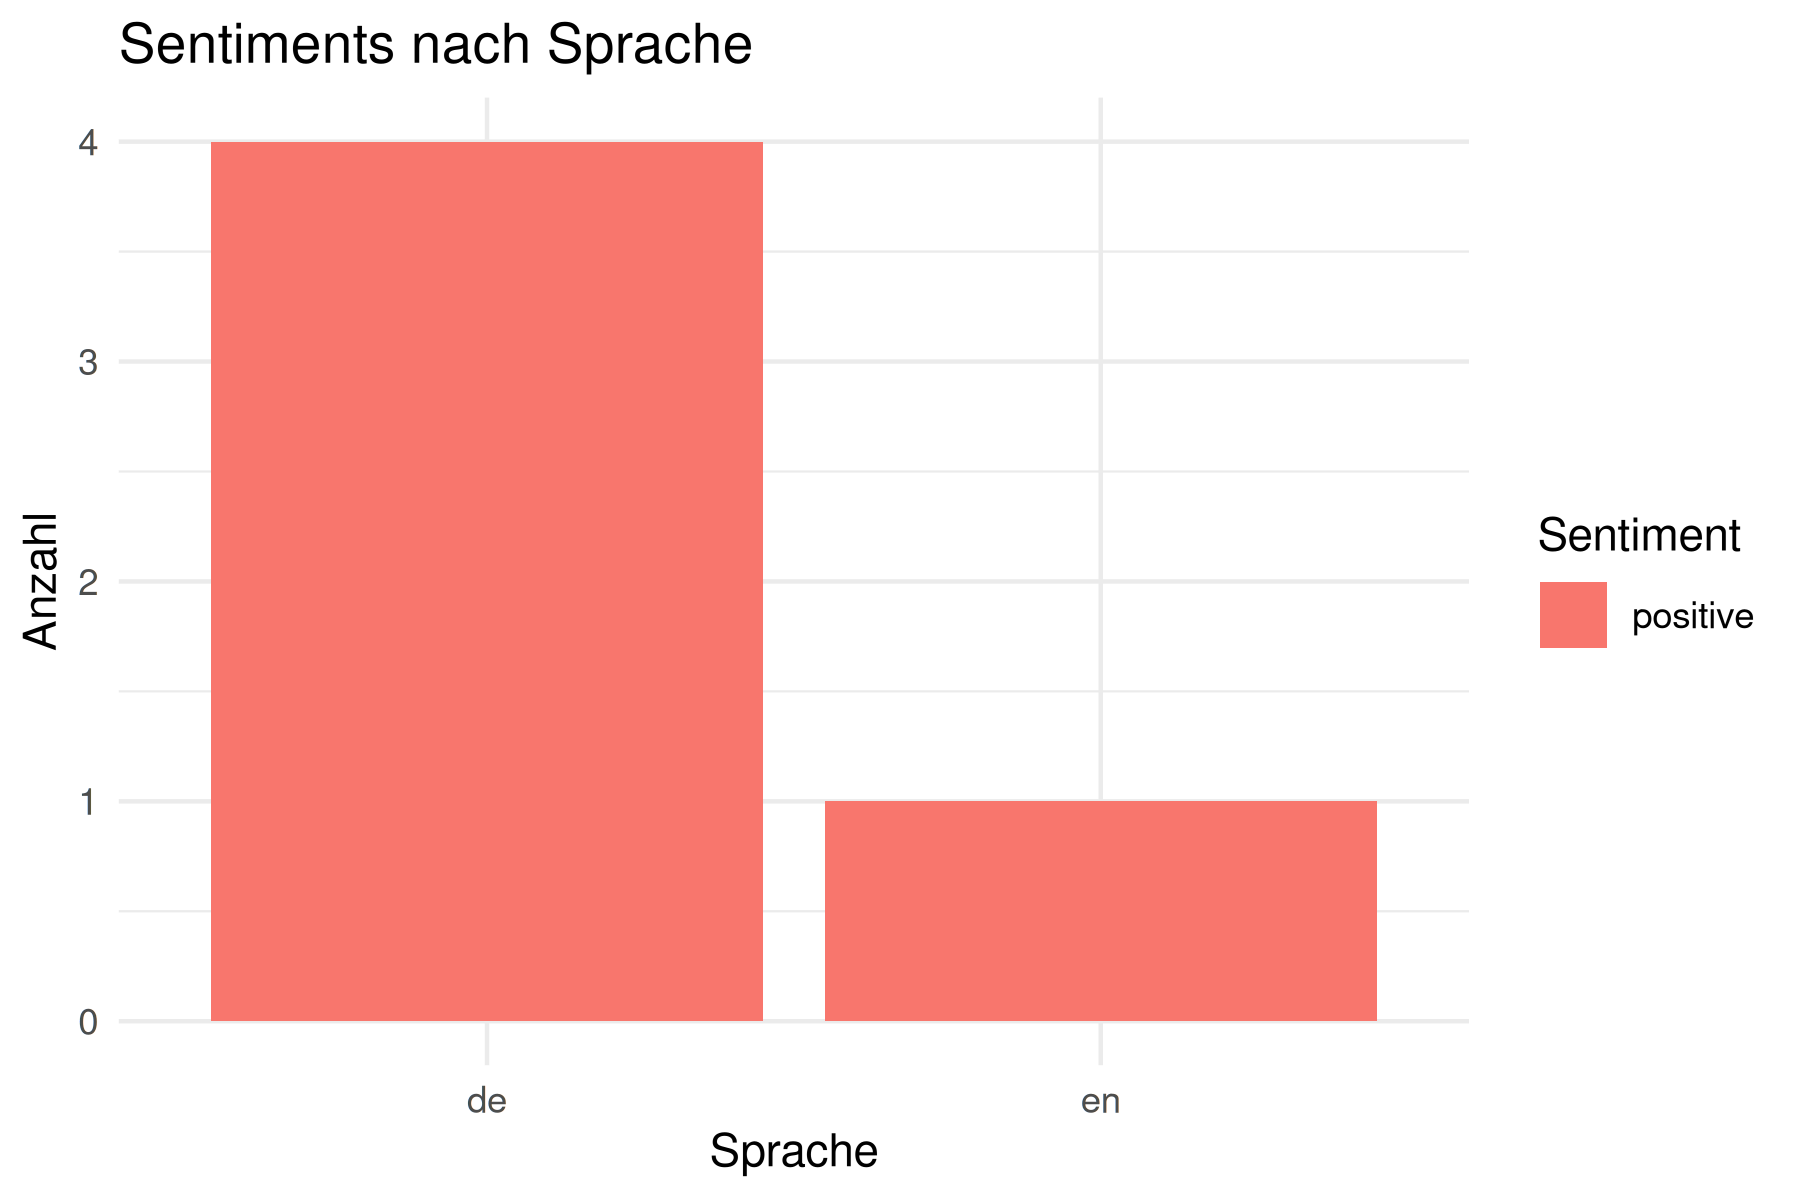
\includegraphics{Analyse_Diagramm2.png}

\subsection{Zufriedenheit mit
Lernmaterialien}\label{zufriedenheit-mit-lernmaterialien}

Das zur Verfügung gestellte Lernmaterial wird überwiegend positiv
bewertet. Einige Studierende wünschen sich jedoch mehr ergänzende
digitale Ressourcen und aktuelle Inhalte.

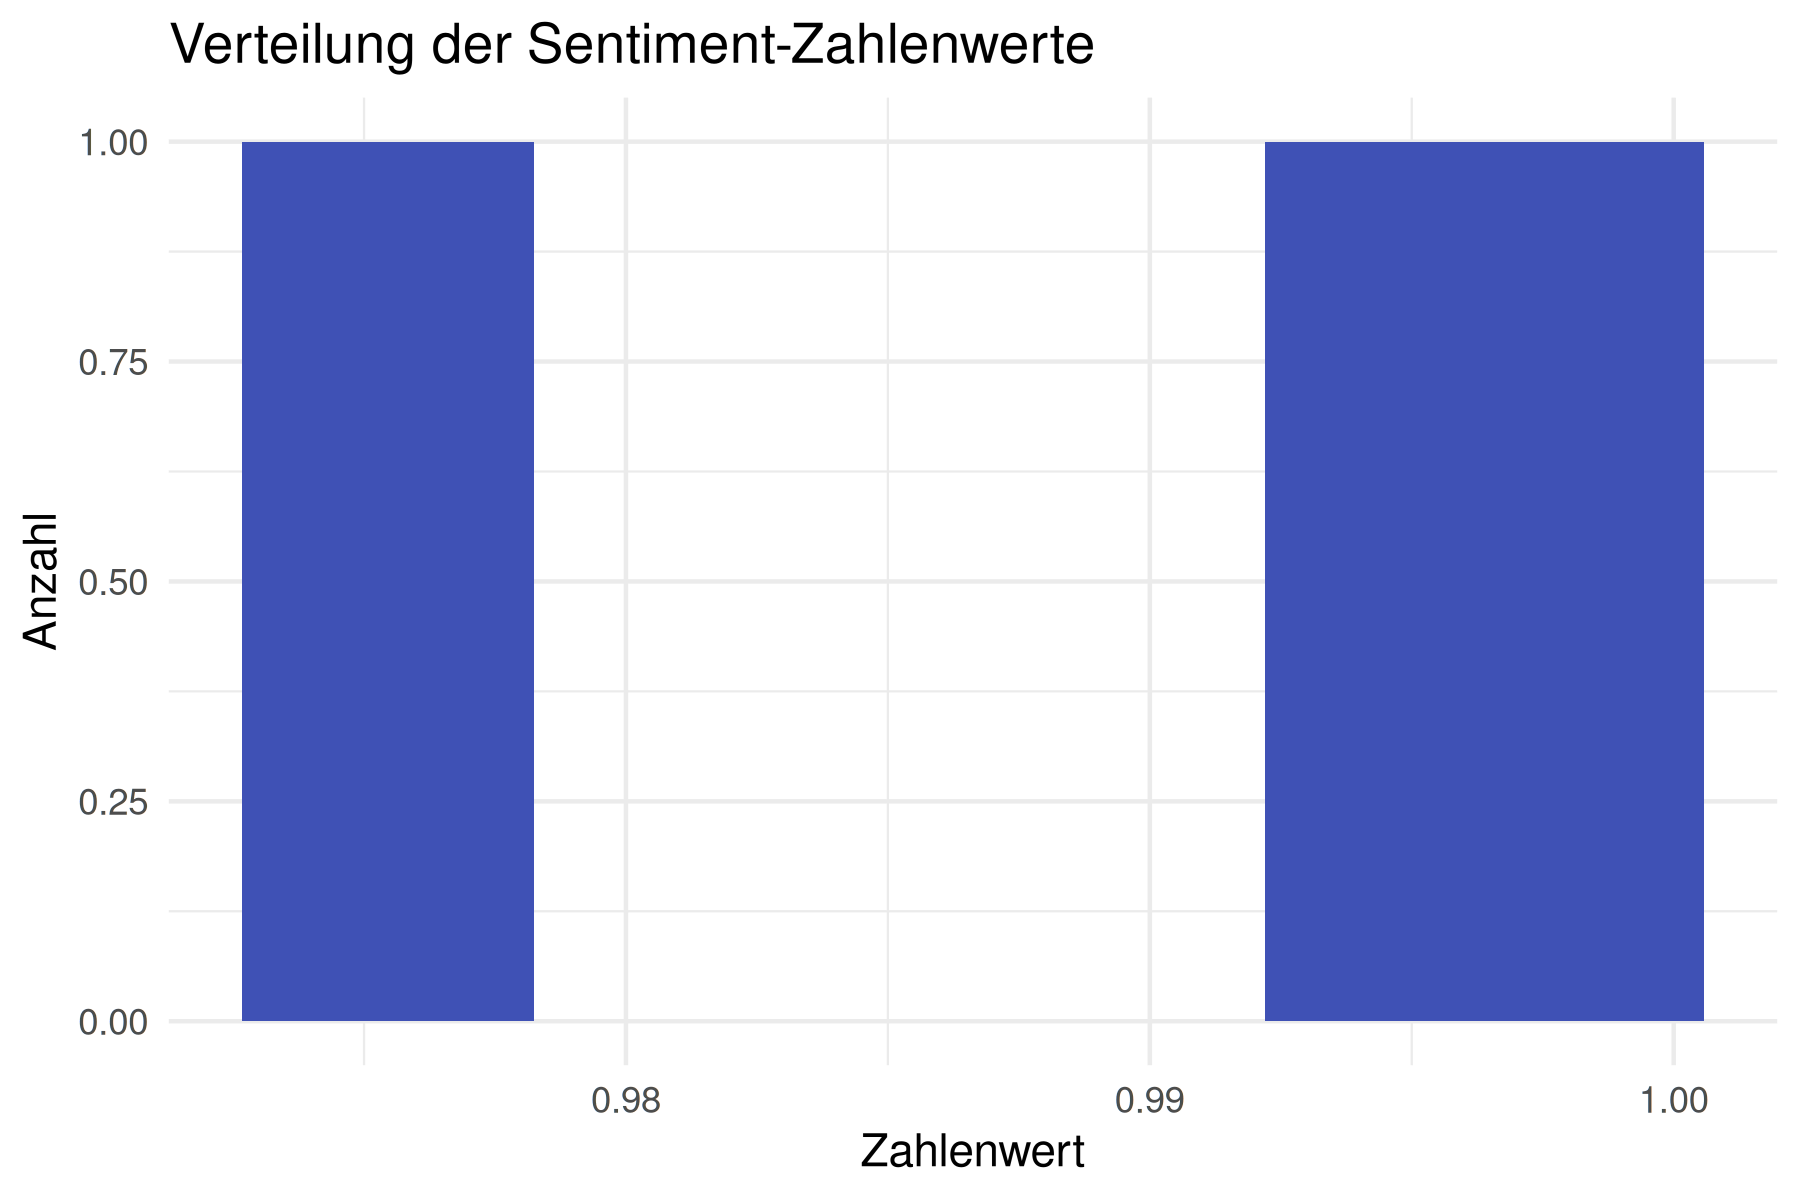
\includegraphics{Analyse_Diagramm3.png}

\subsection{Fazit}\label{fazit}

Das Feedback zeigt eine hohe Zufriedenheit, weist jedoch auf Potenziale
in Interaktivität, Betreuung und digitalen Ressourcen hin.

\end{document}
